%!TEX root = ../thesis.tex
\begin{savequote}[75mm]
In an Agile project the team takes care of the tasks and the project leader takes care of the team.
\qauthor{Jim Highsmith}
\end{savequote}

% todo Domanda (la risposta aiuta anche per la presentazione): Avendo chiarito il contesto Agile, Jira e Confluence sn le unice risposte? 
%todo Quel che intendo dire e' che nella parte di background tecnologico e' utile esporre vari approcci (hai fatto un studio di dominio) e un eventuale piccolo confronto (non indispensabile per una tesi 3-ennale) e poi concludi che questi strumenti sono stati scelti perche... anche semplicemente Imposti dal contesto aziendale.
%todo Pensaci.. non farei ora questa modifica - vediamo alla fine. Pero preparati un argomento simil. per la presentazione. Dimostra maturita'.

\chapter{Jira and Confluence: the essentials}
\label{chapter_4}
	Now that the main concepts of Agile and it's derivatives have been explained, let's understand how Jira and Confluence work.
	These are proprietary tools developed and maintained by the Australian company Atlassian.
	\begin{figure}[H]
		\centering
		
\includegraphics[width=.7\textwidth]{resources/atlassian_logo}\\
		\caption{The logos of \textit{Atlassian}, \textit{Jira}, \textit{Confluence} and \textit{Jira Service Desk}}
	\end{figure}
	Jira is an Issue Tracking System that was first released in 2002, it's name is a truncation of \Quote{Gojira}, the Japanese word for \Quote{Godzilla}.
	This is a reference to another ITS that was dominating the market at the time, \Quote{Bugzilla}.
	At the time of writing, the main competitors of Jira are other software like Redmine, VersionOne, PivotalTracker, Workzone or integrated ITSs in repositories like GitHub's or GitLab's issue trackers\cite{jira-alternatives}.\\
	Athonet's previous choice was Redmine because it is open source (this implies it doesn't need a paid license), it has a medium-large community of people that use it and maintain it behind and the plugins allow the integration with other internally used tools like repositories or software for reporting customer requests.
	\begin{figure}[H]
		\centering
		
\includegraphics[width=.6\textwidth]{resources/redmine_logo}\\
		\caption{\textit{Redmine}'s logo}
	\end{figure}
	Confluence, on the other hand, has been designed as a collaboration platform for sharing knowledge like documents, product specifications, meeting notes and can be used as a wiki for internal use or for releasing information to the clients.\\
	Atlassian released the first version of Confluence in 2004, saying its purpose was to create \Quote{an application that was built to the requirements of an enterprise knowledge management system, without losing the essential, powerful simplicity of the wiki in the process}\cite{theserverside}.\\
	Since the first releases of these products, Atlassian has developed and acquired new tools like \Quote{Bamboo}, \Quote{Clover}, \Quote{Crowd}, \Quote{Crucible}, and \Quote{FishEye}, all orientated towards collaboration, content sharing, issue tracking, time scheduler, etc.\\
	Both Jira and Confluence are written in Java.

\section{What can these tools do}
	These tools are made to be flawlessly integrated with one another, not only because they are made by the same company but they are strictly correlated in their intents.\\
	Integrating an Issue Tracker with a platform able to share documents and thoughts allows a more granular analysis of project requirements.
	This means that the company can store meeting notes and documents related to the project in Confluence, and when they are ready to move into the development phase, convert them to Issues inside Jira.\\
	Plugins can extend by far the usage and integration with other tools and the Atlassian Marketplace \cite{marketplace.atlassian} is full.
	Although there is a license that has to be paid, if used correctly this software can allow the company to save money that could otherwise be lost in badly managed resources like time, documentation and even people.\\
	Let's understand them better.
	\subsection{Jira}
		Over the years Jira has become such an important software that Atlassian had to separate it in three specialized components, each with its own scope.
		Here is a table from Jira's official documentation \cite{server_jira+jsd_product-changes} that contains all the major differences:
		\begin{figure}[H]
			\centering
			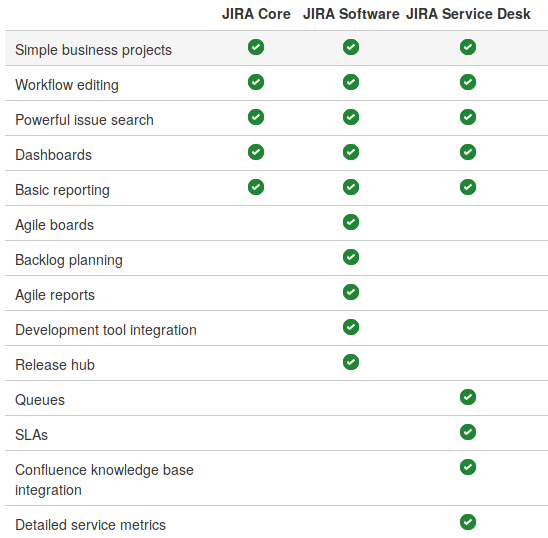
\includegraphics[width=.8\textwidth]{resources/jira_type}\\
			\caption{Differences between \textit{Jira Core}, \textit{Jira Software} and \textit{Jira Service Desk}}
		\end{figure}
		The three editions of Jira have the same look and feel to provide a consistent project experience, but there are some differences that characterizes these standalone products \cite{what-are-the-differences}.
		\subsubsection{Jira Core}
			The core version is a \textit{business oriented} project management software for general team project collaborations and workflow approvals of not technical tasks that can eventually be related with developers' issues.
			It's targeted users are non technical teams like the business, legal, operations and marketing departments.
			
		\subsubsection{Jira Software}
			Its purpose is to plan and track the trend of the project by managing releases and creating reports from real time data in order to improve the teams' performance.
			Each project can have its own workflow and can be integrated with other Atlassian tools for better coverage.
		
		\subsubsection{Jira Service desk}\label{subsec:service_desk}
			This software's main purpose is to handle customer requests and provide them with a user friendly help center, that, in combination with Confluence, can create a rich navigable knowledge base.
			It can be integrated with Jira Software so IT and developer teams can collaborate on one platform.

		\subsubsection{Jira Portfolio Plugin}\label{subsec:portfolio}
			Portfolio \cite{portfolio} is an add-on for Jira Software that enables teams to build plans and track progress.
			Its main purpose is creating real time roadmaps that can include issues, at various levels by applying filters to see only the interesting ones. 
		
	\subsection{Confluence}
		As described earlier, Confluence is a collaboration platform.
		It allows to create spaces of different categories that can be associated with Jira projects.
		There are many different space types (like knowledge base, documentation, software project, etc.) that contain templates used for creating documents.
		\begin{figure}[H]
			\centering
			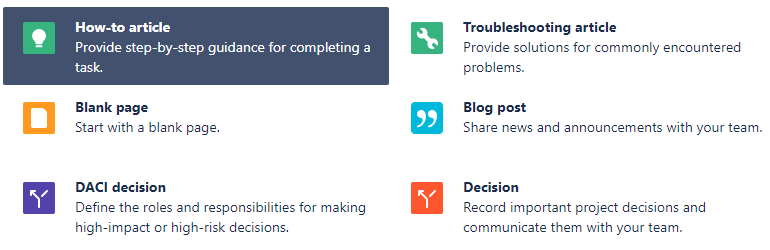
\includegraphics[width=\textwidth]{resources/Annotation2019-07-24180136}\\
			\caption[Some custom templates for Confluence documents]{Some of the custom templates for documents that can be redacted in Confluence}
		\end{figure}
		Companies use Confluence to create public wikis for their customers, e.g. Akraino \cite{akraino}.
		
\section{Key concepts for Jira}\label{sec:concepts}
	Jira has its own terminology that needs to be understood in order to completely master the software.
	The key terms that must be known, according to Jira's guidelines\cite{key-terms-to-know} are:
	\begin{itemize}
		\item \textbf{Issues}: a work item of any type or size that is tracked from creation to completion
		\item \textbf{Projects}: a collection of issues that are held in common by purpose or context
		\item \textbf{Workflows}: represent the sequential path an issues takes from creation to completion
	\end{itemize}
	\begin{figure}[H]
		\centering
		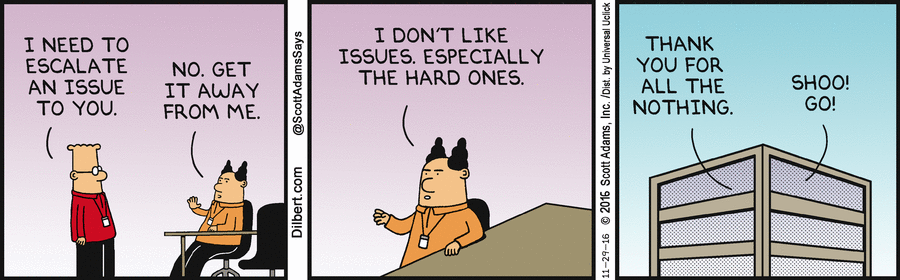
\includegraphics[width=\textwidth]{resources/issues}\\
		\caption{Dilbert on issues}
	\end{figure}
	
\section{How Athonet uses these tools}
	As anticipated, Athonet has chosen Atlassian's Jira and Confluence because they need a single solution that is coherent and that could provide them an unique access for all the company figures to the projects and their related documentation.
	Plus, Jira was also used in the past by some employees at their former company, so there was more familiarity compared to other tools.\\
	Although Confluence's potentials as a documentation writing software, it will be impossible to eliminate the use of Microsoft Office programs (Word, PowerPoint, Excel) to share documents, presentations and other content with clients.
	This is because of their simplicity and massive use for producing records in a fast and user friendly way.\\
	These tools can become complex, it is necessary to understand the scenario they can be used in and make a plan for transitioning from the old software.\\
	It is important for the company to adapt the tools for it and not change their entire way of working to accommodate to the new software.
	\subsection{Development} 
		Compared to Redmine Jira has many more useful functionalities and on top of that it has a richer User Interface (UI).
		\begin{figure}[H]
			\centering
			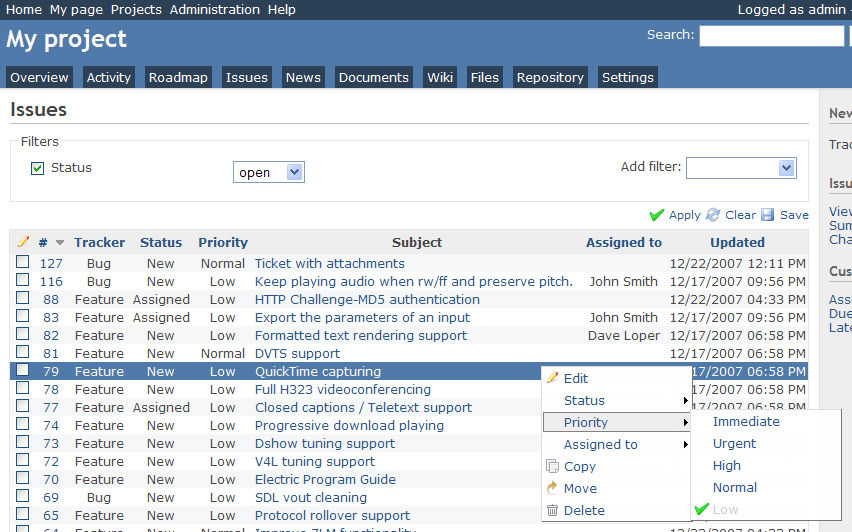
\includegraphics[width=\textwidth]{resources/redmine_screennn}\\
			\caption{Example of Redmine's interface}
		\end{figure}
		The development team will be the one that will use it the most, and because of that it is important that it can integrate with GitLab.
		With the GitLab Listener plugin \cite{gitlab-listener} Developers can interact with Jira's issues from the messages in the repository's operation.
	
	\subsection{Management} 
		The most important feature the management department needed was the live roadmap.	
		It's a key element for this kind of company since it allows to keep an eye the trend in development and manage the releases.
		Jira's Portfolio allow to apply filters that can display a different granularity on what is shown, this means that it can be used at more levels in the company's hierarchy.\\
		With the kind of tools currently in use it's not possible to have such a smooth integration.
	
	\subsection{Client interaction} 
		Although Service Desk would be the ideal software to allow the interaction with clients, Athonet has not yet thought of using it in such a way, but there is the possibility to do so in the future.
		
	\subsection{Internal documentations}
		Confluence substitutes the multiple wiki software that were previously installed, allowing an integration with Jira and offering a richer experience for the employees.
	
\section{The Atlassian Community}\label{sec:atlassian_community}
	Athonet has chosen wisely to buy the licenses Jira and Confluence over other tools and over creating their own internal solution, which would have meant reinventing the wheel.\\
	Compared to other tools, Atlassian has built a large community around its products, allowing people to ask and answer questions on a blog, request for new features, open tickets, view the dates and changelog of next releases and report bugs.
	\begin{figure}[H]
		\centering
		\makebox[\textwidth][c]{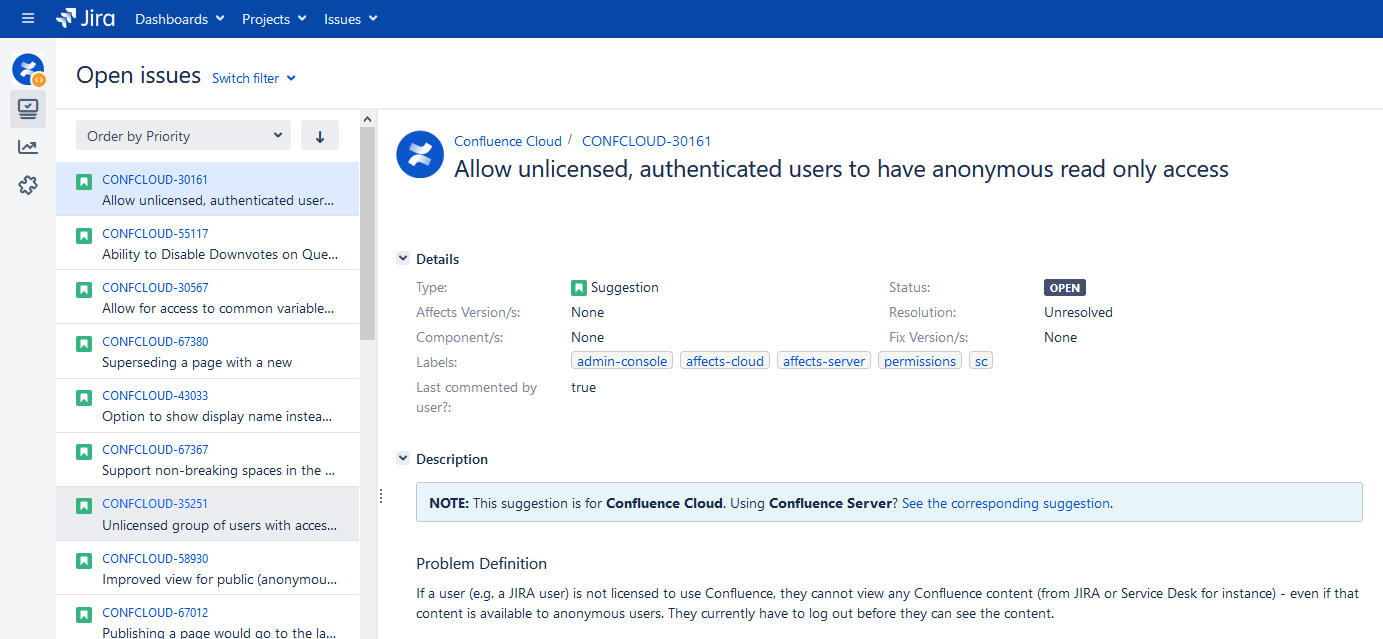
\includegraphics[width=1.1\textwidth]{resources/confluence_documentation_issues_1}}%
		\caption{The issues related with Jira and Confluence are handled by a dedicated Jira Cloud instance}
	\end{figure}
	This allowed me to easily find not only the resolutions to some implementation problems that occurred during the installation, but also tips on how to better configure the software.

